\chapter{Introduction}
\label{introchap}
In this paper we present the Lifetime-Limited Memory (LLM) network to make specific use of the temporal aspects of event sequence data. Different forms of recurrent neural networks have been implemented sequence data (specifically the Long Short-Term Memory (LSTM)\cite{LSTM} network is particularly prolific), but they do not impose specific structure to the networks treatment of temporal data. The LLM is a recurrent neural network that explicitly decays memory at different exponential rates based on the time between events. This temporal dynamic should more closely model human behavior and memory than an unstructured temporal dimension allows. The different decay rates of memory traces should allow the LLM to learn data patterns occurring at many different timescales. The network uses this cell memory to either make a prediction at each step, or classify the sequence as a whole. 
\\\\
Event sequence data, which the LLM takes as input, is formatted as an ordered list of paired labels and timestamps. For instance, one could represent someone's text message history as an event sequence, where the recipient is the label for the event, and the time the message was sent as the timestamp. It can also be beneficial to represent the timestamp as time since the last event, as we use in the context of our model. There is a graphical representation of this data in figure \ref{fig:Event_seq}

\begin{figure}
    \centering
    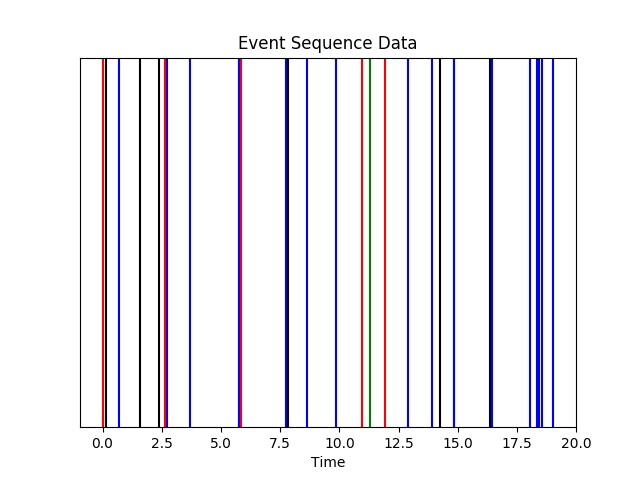
\includegraphics[width=1.0\textwidth]{figures/Event_Sequence.png}
    \caption{Event Sequence Data}
    \label{fig:Event_seq}
    An example an event sequence with 4 different event types
    
\end{figure}
\textit{ }\\ One can easily see why a network that uses event sequence data could be applicable to a variety of tasks. Consider, for instance, that an advertising company provides you with a shopping history of a customer, and want to be able to best recommend a product to them at any given time. This network would be ideal for this task. Or perhaps, given a user's browsing history, you wanted to classify some aspect of the user, like whether they are a parent or not. This type of architecture could be very useful for many types of tasks attempting to gain insight into human behavior, and the LLM will hopefully have a memory highly capable of mimicing that of a human. 